\chapter{Proposta}\label{cap4}

\section{Usuários}

Pessoas e instituições estão se afastando cada vez mais de impressões e se aproximando de livros eletrônicos. Os e-books estão fazendo sucesso e estão cada vez mais sendo utilizado pelos editores para tornar disponíveis livros em formato eletrônico. Eles oferecem benefícios para os leitores incluindo a redução de danos ao meio ambiente, a portabilidade, o peso leve e ao reforço da capacidade de referência. Mas, para alguns leitores, e-books oferecem ainda mais: a sua primeira oportunidade de desfrutar da leitura. Essa pessoas com algum tipo de limitação, seja cego ou com baixa visão, pessoas com dislexia ou outras dificuldades de aprendizagem ou ainda que não conseguem segurar ou mudar a página de um livro encontram enormes dificuldades para ler livros impressos e, dependendo do caso, tal prática torna-se impossível \cite{chronicle}.

Neste contexto este mecanismo de semântica e ontologia proposto, poderia auxiliar os usuários de audiobooks a possuírem maior mobilidade e conforto ao dispor destas tecnologias.

\section{Terminologias Existentes}

\subsection{Ontologias Existente}
Ontologias para a organização de \textit{audiobooks} são raras. Porém há uma grande similaridade entre ontologias para livros e para \textit{audiobooks}, uma vez que que tanto o livro quanto o áudio descrevem o mesmo conteudo. Mundando unicamente a forma que disponibilizam esse material. Dessa forma, a ontologia usada - nesse trabalho - para organizar ontologicamente um audiobook foi baseada uma ontologia desenvolvida por Naveen Kumar no intituto \textit{Ambedkar Institute of Advanced Communication Technologies}. 

A ontologia desenvolvida em Ambedkar deve cobrir uma ampla quantidade de informações e deve ter a capacidade para especificar as informções de formar a tornar mais eficas a pesquisa\cite{ontologybook}. A figura 2 mostra a abstração basica dos conceitos relacionados à livros e as relações semânticas. 

Existem basicamente quatro relações entre os conceitos: a relação de herança, relação de instância, relação parte-todo e relação sinoníma. A Relação de herança revela a relação de inclusão entre conceitos, ou seja, um subi-conceito é uma espécie de conceito pai, como por exemplo: ``Ruby of Rails'' é uma espécie de ``livro técnico'', em que ``livro técnico'' é um conceito pai, e ``Ruby of Rails'' é a sub-classe. A relação de instância é a relação da existência especifica de um conceito, como ``livro departamento de TI'' é uma instância de ``livro computador''. Relação parte-todo expressa um conceito que faz parte de um outro conceito, como ``manual de laboratório'' é parte do ``livro departamento de eletrônica''.

Não há informação semântica rica descrito explicitamente na ontologia. Podemos conhecer a partir da Figura 2 que o Java é um livro departamento CSE de livros de informática, e as pessoas podem chamá-lo pelo nome de ``OAK''. RDF (Resource Description Framework) e RDFS (RDF Schema) é um modelo de dados e mecanismo de apoio para a representação de meta-dados de esquemas \cite{rdf}, e é uma linguagem de representação de ontologias. RDF é um padrão baseado em XML para descrever recursos que existem na web, intranets e extranets. RDFS é usado para criar vocabulários que descrevem grupos de recursos RDF relacionados e as relações entre esses recursos. 


 \begin{figure}[ht]
	\centering
		\includegraphics[keepaspectratio=true,scale=0.5]{figuras/ontology.eps}
	\caption{Uma pequena parte da ontologia no dominio de livros.}
	\label{lanctocalivros}
\end{figure}

\section{Descrição do Ambiente Web}
Audiobook, basicamente são livros narrados. Ou seja, são gravações dos conteúdos de livros, cujo o mesmo é lido. Estes audiobook posuem diversos formatos informacionais, como MP3 e WMA, entre outro, podendo ser pagos ou gratuitos, dependendo da plataforma à qual os audibooks, encontram-se disponíveis.
Ideal para os leitores que gostam de praticar o habito da leitura, porém não dispõem o tempo necessário para exercer esta atividade. Estes audiobooks, podem possuir diversas funcionalidade que enriquecem a esculta, como efeitos sonoros, variações no tom de voz, entre outros meios que evitam a ociosidade na esculta.
Possuem uma quantidade de exemplares no idioma português relativamente baixa, porém possuem uma grande variedade de conteúdo internacional, principalmente no idioma inglês, um dos maiores mercados de audiobooks disponível.

\chapter{Descrição sobre o Protégé}\label{cap4}

A ferramenta Protége é um software de código aberto desenvolvido pelo “Stanford Center for Biomedical Informatics Research” da universidade “Stanford University School of Medicine”, o qual fornece uma interface gráfica com um conjunto de ferramentas para o desenvolvimento de ontologias \cite{Protege}.

A ferramenta possibilita dois tipos principais de trabalho, sendo estes o desenvolvimento online através do “WebProtégé” ou o desenvolvimento através de um software instalado localmente o “Protégé Desktop”, ambas gratuitas com um amplo conjunto de tutoriais disponíveis no site da empresa.

Este projete se concentrara na versão para desktop Protege-5.0.0-beta-17, está versão encontra-se em desenvolvimento, construída para fins de teste, não possuindo nenhum tipo de lançamento oficial disponível, na páginas de download da ferramenta. É possível obter uma cópia do código fonte da ferramenta através do repositório no github através do link: \cite{GIT}.

A ferramenta oferece suporte para a criação das principais funcionalidades de uma ontologia, como a criação de classes com suas respectivas hierarquias. A definição de relacionamentos entre os dados, a definição de propriedades dos objetos. Além de possuir a possibilidade de visualização do trabalho desenvolvido através de gráficos gerados pela mesma.

 \begin{figure}[ht]
  \centering
    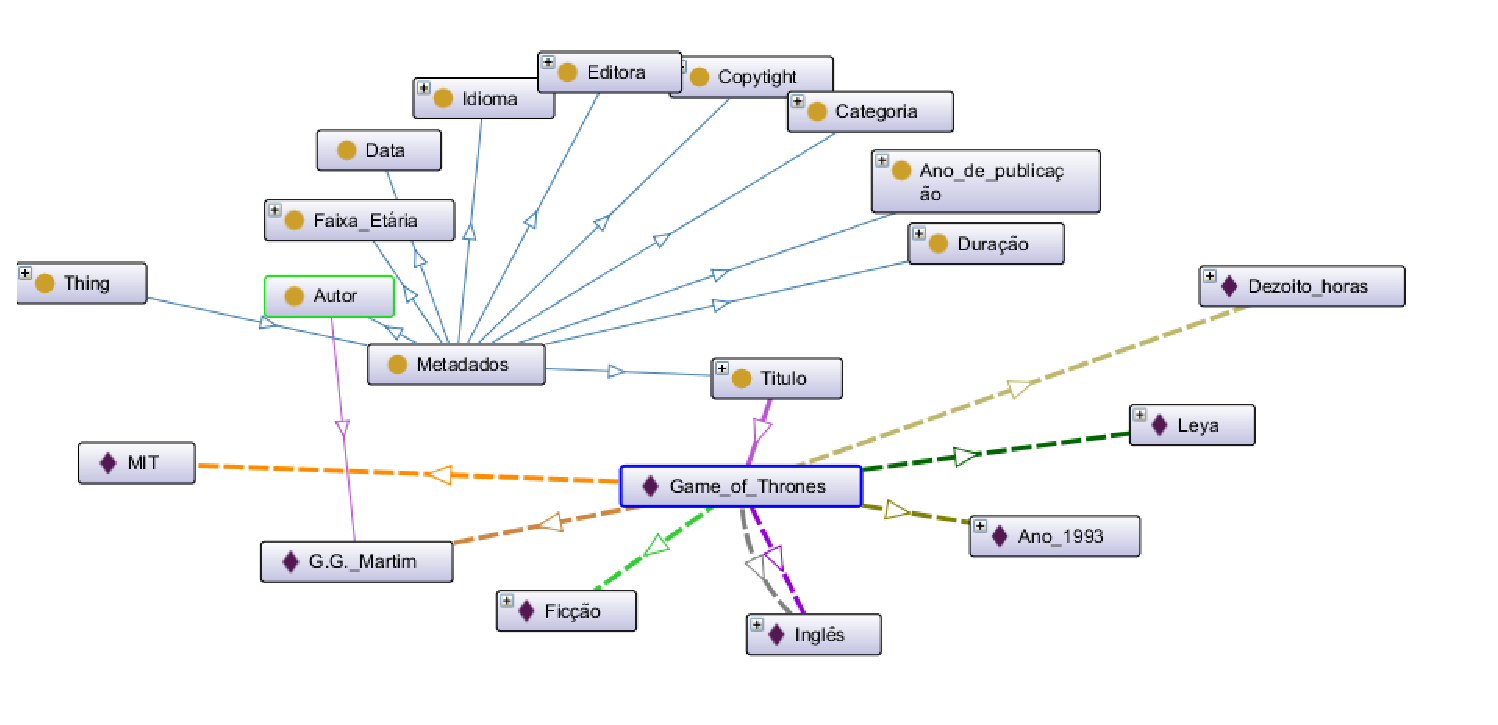
\includegraphics[keepaspectratio=true,scale=0.5]{figuras/protege.eps}
  \caption{Gráfico gerado com a ferramenta Protégé, com relacionamentos referentes ao audioBook Game of Thrones.}
  \label{fig:protege}
\end{figure}

\section{Descrição da ontologia criada}

A ontologia desenvolvida nesse trabalho é apenas ilustrativa, uma vez que a modelagem não contou com participação de nenhum especialista no assunto. O que será apresentado a seguir é apenas uma ideia inicial para a equipe de realizar o projeto descrito nesse trabalho. 

\subsection{Modelagem de classes}

Para chagar-se às classes implementadas no projeto, foi utilizada a técnica de \textit{card sorting} - \textit{Card sorting} é um método usado para facilitar design ou validadar a arquitetura da informação. Em uma sessão de card sorting, os participantes organizam os tópicos em categorias que fazem sentido \cite{cardsorting} - após essa atividade, chegou-se a algumas classes, mostradas a seguir.

\begin{description}
  \item[Marcações] \hfill \\
  Uma vez que o objetivo da ontologia é a estruturação semântica de um audiobook com suporte a \textit{tags}, está classe representa as marcações de conteúdo ao decorrer do áudio.
  \item[Autor] \hfill \\
  Uma das principais caracteristicas de audiobooks são os autores, ou seja, é importante ter essa informação semânticamente.
  \item[Editora] \hfill \\
  Classe que descreve a editora do audiobook.
  \item[Idioma] \hfill \\
  Classe que descreve a idioma do audiobook.
  \item[Faixa Etária] \hfill \\
  Classe que descreve a idade recomendavel para o público do audiobook, assim podemos diferencias conteúdo para adultos de conteúdos de crianças.
  \item[Copyright] \hfill \\
  Classe que descreve os diretiros sobre o audiobook.
\end{description}


\subsection{Mapa mental}

Para a estruturação das classes e informações da ontologia, foi executado a técnica de mapa mental. A ferramenta xMind foi utilizada para a implementação da técnica. A figura \ref{fig:xmind} é o resultado dessa atividade.

\begin{figure}[H]
  \centering
    \includegraphics[keepaspectratio=true,scale=0.5]{figuras/xmind.eps}
  \caption{Mapa mental da ontologia de audiobooks.}
  \label{fig:xmind}
\end{figure}

Com a atividade de mapa mental foi possivel identifacar novas classes, como por exemplo a classe “Metadados”. Essa classe é a classe pai de todas que praticamente todas as outra classes e possui propriedades fundamentais para a descrição semântica do audiobook. Uma das propriedades fundamentais dessa classe é o titulo e a descrição. Essa propriedades caracterizam várias \textit{querys} do usuário, sendo de grande influência no resultado da busca.

\subsection{Implementação no Protegê}

Com a estruturação do mapa mental, a implimentação no protegê se torna bem prática, uma vez que esse processo se torna apenas em transcrever a informação do mapa metal para a ferramenta protegê. 

A figura \ref{fig:protege} é o resultado da modelagem da ontologia após a criação de algumas instâncias para teste e exemplo. A figura \ref{fig:rdf} é uma parte do RDF gerado pela ferramenta e é em si a ontologia.

\begin{figure}[H]
  \centering
    \includegraphics[keepaspectratio=true,scale=0.5]{figuras/xmind.eps}
  \caption{RDF da ontologia de audiobooks}
  \label{fig:rdf}
\end{figure}

